\documentclass[../../main.tex]{subfiles}
 
\begin{document}

\section{Лекция 7. 27 ноября 2019 г.}

\textit{Обозначение.} $(X_i)_{i \in I}, (Y_i)_{i \in I}$ — семейства множеств, $\left( f_i \colon X_i \to Y_i \right)_{i \in I}$ — семейство отображений.

\defn (декартово) произведение семейства $(f_i)$ отображение $\prod_{i \in I} f_i \colon \prod_{i \in I} X_i \to \prod_{i \in I}Y_i, (x_i)_{i \in I} \mapsto \left( f_i(x_i) \right)_{i \in I}$

\textbf{Предложение.} Пусть $(X_i)_{i \in I}, (Y_i)_{i \in I}$ — семейства топологических пространств, $( f_i \colon X_i \to Y_i)_{i \in I}$ — семейство непрерывных отображений.

Тогда $\prod f_i \colon \prod X_i \to \prod Y_i$ — непрерывно.

\textit{Доказательство:} Обозначим $X$ — $\prod X_i, Y = \prod Y_i, f = \prod f_i$

\begin{minipage}{0.20\linewidth}

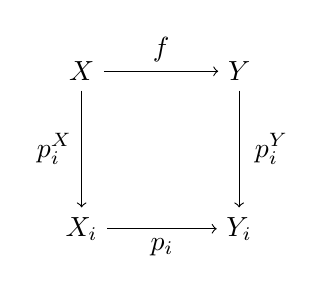
\begin{tikzpicture}[node distance=2cm, auto]
\node (X) {$X$};
\node(Y) [right of=X] {$Y$};
\node (X1) [below of=X] {$X_i$};
\node (Y1) [below of=Y] {$Y_i$};
\draw[->](X) to node {$f$}(Y);
\draw[->](X) to node [left] {$p^X_i$}(X1);
\draw[->](X1) to node [below] {$p_i$}(Y1);
\draw[->](Y) to node [right=0.5ex] {$p^Y_i$}(Y1);
\end{tikzpicture}
\end{minipage}
\begin{minipage}{0.8\linewidth}
$f$ непрерывно $\lra p^Y_i \circ f$ непрерывно $\fo i$ (см. свойства инициальной топологии) $\lra f_i \circ p^X_i$ непрывно $\fo i$; а это верно по условию. $\quad \square$
\end{minipage}

\textit{Следствие:} $X$ — топопологическое пространство, $\K = \R$ или $\mathbb{C}$, $C (X) = C(X, \R)$.

Тогда $\fo f,g \in C(X) \quad f + g \in C(X)$ и $fg \in C(X)$

Если $f(x) \neq 0 \; \fo x \in X$, то $\frac 1 f \in C(X)$

\textit{Доказательство:}

%\begin{tikzpicture}[node distance=2cm, auto]
%\node (X) {$X$};
%\node (X1) [below of=X];
%\node(XTX) [right of=X] {$X \times X$};
%\node (KK) [right of=XTX] {$\K \times \K$};
%\node (K) [right of=KK] {$\K$};
%\node (K1) [below of=K];
%\draw[->](X) to node [above] {$\Delta$} node %[below] {$x \to (x,x) \text{непр.}$}(XTX);
%\draw[->](XTX) to node {$p^X_i$}(KK);
%\draw[->](KK) to node {$p_i$}(K);
%\draw[-](X) to (X1);
%\draw[-](X1) to (K1);
%\draw[->](K1) to (K);
%\end{tikzpicture}

\textbf{Предложение:} Топологическое пространство $X$ — хаусдорфово $\lra$ диагональ $D_X = \left\{ (x, x) \colon x \in X \right\} \subset X \times X$ замкнута в $X \times X$

\begin{minipage}{0.2\linewidth}
%\begin{tikzpicture}[node distance=2cm, auto]
%\node (X);
%\node(Y) [right of=X] 
%\node (X1) [below of=X] 
%\node (Y1) [below of=Y]
%\draw[->](X) to node {$f$}(Y);
%\draw[->](X) to node [left] {$p^X_i$}(X1);
%\draw[->](X1) to node [below] {$p_i$}(Y1);
%\draw[->](Y) to node [right=0.5ex] {$p^Y_i$}(Y1);
%\end{tikzpicture}
(картинка квадрата)
\end{minipage}
\begin{minipage}{0.8\linewidth}
\textit{Доказательство:} $D_x$ замк в $X \times X \lra \fo p \in (X \times X) \backslash D_x \; \ex $ окрестность $W$ вида $W = U \times V$ (где $U, V \subset X$ откр.), т.ч. $W \cap D_x = \varnothing$

$\lra \fo x, y \in X$, т.ч. $x \neq y, \ex$ откр $U,V \subset X$, т.ч. $x \in U, y \in V$, и $U \cap V = \varnothing \lra X$ хаусдорфово. $\quad \square$.
\end{minipage}

\textit{Следствие 1.} $X, Y$ — топологические пространства, $Y$ хаусдорфово, $f, g \colon X \to Y$ непрерывно $\Ra \left\{x \in X\colon f(x) = g(x) \right\}$ замкнуто в $X$.

\textit{Доказательство:} Рассмотрим $F \colon X \to Y \times Y, \quad F(x) = \left(f(x), g(x) \right), \quad F$ непрерывно.

$\left\{ x \colon f(x) = g(x) \right\} = F^{-1}\left( D_Y \right)$, а $D_Y$ замкнуто в $Y \times Y. \quad \square$.

\textit{Следствие 2.}  $X, Y$ — топологические пространства, $Y$ хаусдорфово, $f, g \colon X \to Y$ непрерывно.

Пусть $X_0 \subset X$ — плотное подмножество, $f\big|_{x_0} = g\big|_{x_0} \Ra f = g$

\textit{Доказательство:} Множество $S = \left\{ x \in X \colon f(x) = g(x) \right\}$ замкнуто и содержит $X_0 \Ra S = X \quad \square$.

\subsection{Финальные топологии. Дизъюнктные объединения}

$X$ — множество, $( X_i, \tau_i)_{i \in I}$ — семейство топологических пространств; $(f_i \colon X_i \to X)_{i \in I}$ — семейство отображений

\defn \textbf{\textit{Финальная топология}} на $X$, порожденная семейством отображений $(f_i)_{i \in I}$ — это 

$$\tau_{\fin} = \lbrace U \subset X \colon f^{-1}(U) \in \tau_i \; \fo i \in I \rbrace$$

\textit{Замечание:} $\tau_{\fin}$ действительно является топологией на $X$

\textit{Примечание:} Финальная топология на $X_i$, порожденная отображением $\left\{ \varnothing \to X \right\}$ — дискретная топология.

\begin{theo}[(основные свойства финальной топологии)]{thm:main_fin_top}

(1) $\tau_{\fin}$ — самая тонкая топология на $X_i$ , т.ч. все $f_i \colon X_i \to X$ непрерывны
(существует ли самая грубая? Да: антидискретная)\\
(2) Если $Y$ — топологическое пространство, то отображение $g \colon X \to Y$ непрерывно $\lra g\circ f_i$ непрерывно $\fo i$
\end{theo}
\begin{minipage}{0.15\linewidth}
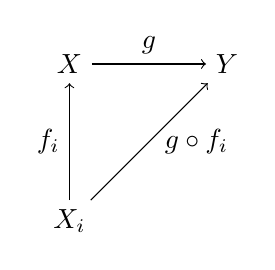
\begin{tikzpicture}[node distance=2cm, auto]
\node (X) {$X$};
\node(Y) [right of=X] {$Y$};
\node (X1) [below of=X] {$X_i$};
\draw[->](X1) to node {$f_i$}(X);
\draw[->](X) to node {$g$}(Y);
\draw[->](X1) to node [right=0.5ex] {$g\circ f_i$}(Y);
\end{tikzpicture}
\end{minipage}
\begin{minipage}{0.85\linewidth}
\textit{Доказательство:} 

(1) $\fo i \in I \; \fo U \in \tau_{\fin} \quad f^{-1}_i(U) \in \tau_{\fin}$ — верно по определению $\tau_{\fin} \Ra f$ непрерывно.

Пусть $\sigma$ — топология на $X$, т.ч. $\fo i \in I \quad f_i \colon X_i \to (X, \varnothing)$ непр

$\fo U \in \sigma \; \fo i \in I \quad f^{-1}_i(U) \in \tau_{\fin} \Ra U \in \tau_{\fin} \Ra \sigma \subset \tau_{\fin}$

(2) $g$ непрерывно $\lra \fo$ откр $V \subset Y \quad g^{-1}(V) \in \tau_{\fin} \lra \fo$ откр $V \subset Y \fo i \in I \;\; \underbrace{f^{-1}_i (g^{-1}(V))}_{(g \circ f_i})^{-1} (V) \in \tau_{\i}$

$\lra  \fo i \in I \quad g \circ f_i \colon X_i \to Y$ непрерывно. $\quad \square$
\end{minipage}

\textit{Упражнение:} $\tau_{\fin}$ — единственная топология на $X$, обладающая свойством (2).

\subsection{Дизъюнктные объединения множеств}

$(X_i)_{i \in I}$  — семейство множеств.

\defn \textit{Дизъюнктное объединение} семейства $(X_i)_{i \in I}$ — множество

$$\bigsqcup_{i \in I} X_i = \left\{(x, i) \colon i\in I, x \in X_i \right\}$$

\textit{Обозначение} $\fo j \in I \quad  q_j \colon X_j \to \sqcup_{i \in I} X_i$; $q_j(x) = (x, j)$ — каноническое вложение $X_j$ в $\sqcup_{i \in I} X_i$.

\textit{Наблюдение:}

(1) $q_j$ — инъекция $\fo j$

(2) $q_i(X_i) \cap q_j(X_j) = \varnothing \; \fo i \neq j$

(3) $\sqcup_{i \in I} X_i = \bigcup_{i\in I}q_i(X_i)$

\textit{Соглашение:} Отождествляем $X_j \subset q_j(X)$ посредством $q_j$

\subsection{Дизъюнктные объединения (несвязные суммы) топологических пространств}

$(X_i)_{i \in I}$ — семейство топ пр; $X = \sqcup_{i \in I} X_i, q_j \colon X_j \to X$ — каноническое вложение $(j \in I)$.

\defn \textit{Топология дизъюнктного объединения} на $X$ — финальная топология, порожденная семейством $(q_i \colon X_i \to X)_{i \in I}$ канонических вложений.

Таким образом $U \subset X$ откр $\lra U \cap X_i$ открыто в $X_i \fo i \in I$

\begin{theo}[(универсальное свойство дизъюнктного объединения)]{thm:un_diz}

$(X_i)_{i \in I}$ — семейство топологических пространст, $Y$ — топологическое пространство, $X = \sqcup_{i \in I} X_i$.

Тогда для любого семейства непрерывных отображений $(f_i \colon X_i \to Y)_{i \in I}$ существует единственное непрерывное $f \colon X \to Y$, т.ч. диаграмма (D) коммутативна $\fo i \in i$

\begin{minipage}{0.2\linewidth}
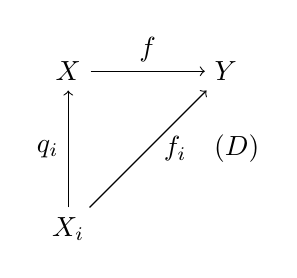
\begin{tikzpicture}[node distance=2cm, auto]
\node (X) {$X$};
\node(Y) [right of=X] {$Y$};
\node (X1) [below of=X] {$X_i$};
\draw[->](X1) to node {$q_i$}(X);
\draw[->](X) to node {$f$}(Y);
\draw[->](X1) to node [right=0.5ex] {$f_i \quad (D)$}(Y);
\end{tikzpicture}
\end{minipage}
\begin{minipage}{0.75\linewidth}

\textbf{\\Доказательство:} 

зададим $f \colon X \to Y$ так:
$$f(\left (x, i) \right) = f_i (x) \quad (\fo i \in I, \fo x \in X_i) \quad (*)$$

Отображение $f$ делает (D) коммутативной и является единственным отображением с этим свойством (т.к. (*) эквивалентно $f(q_i(x)) = f_i(x)$).\\ Непрерывность $f$ из теоремы 1 $\square$. 
\end{minipage}

\end{theo}

\subsection{Связные топологические пространства}

\defn Топологическое пространство $X$ \textit{\textbf{связно}} $\lra X $ не представимо в виде $X = U \cup V$, где $U, V$ открыты, непусты и $U \cap V = \varnothing$

$X$ \textit{несвязно}, если оно не является связным

Подмножество $Y \subset X$ \textit{связно} $\lra$ оно связно как топологическое пространство в индуцированной топологии.

\textit{Наблюдение:} $X$ связно $\lra X$ не представимо в виде $X = A \cup B$, где $A, B$ замкнуты, непусты и $A \cap B = \varnothing$

$\lra$ не существует подмножества $A \subset X, A \neq X, A \neq \varnothing$, открытого и замкнутого одновременно.

\textbf{Пример.} Дискретное пространство, состоящее более чем из 1 точки, несвязно.

\textbf{Пример 2.} Антидискретное пространство связно.

\textbf{Пример 3.} $\R \backslash \{0\}$ несвязно, т.к. $\R \backslash\{0\} = (-\infty; 0) \cup (0;\; +\infty)$.

\textbf{Пример 4.} (картинка) $\overline{B_1}(0,0)\cup \overline{B_1}(0, 3) \subset \R^2$ — несвязное. 

\textbf{Пример 5.} Любое подмножество $A \subset \Q$ (с топологией, индуцированной из $\R$), состоящее более чем из одной точки, несвязно.

Действительно: пусть $a, b \in A, a < b. \ex $ иррац. $c \in \R$, т.ч. $a < c < b$

$U = A \cap (-\infty;\; c), V = A \cap (c,\; +\infty) \Ra U, V$ откр. в $A, U \cap V = \varnothing, U \cup V = A$. 

\end{document}